% JAC-ECC 2026 IEEE Conference Paper Draft (DOUBLE-BLIND SUBMISSION)
% Neuro-Symbolic Breast Cancer Diagnosis Using DeepProbLog and Medical Knowledge
%
% Compile with: pdflatex main && bibtex main && pdflatex main && pdflatex main
%
% CAMERA-READY: After acceptance, restore the real author block below and
% re-add acknowledgments/funding if desired. Do not include those in review.
%
\documentclass[conference]{IEEEtran}

\usepackage{amsmath,amssymb,amsfonts}
\usepackage{graphicx}
\usepackage{cite}
\usepackage{booktabs}
\usepackage{url}
\usepackage{xcolor}
\usepackage{tikz}
\usetikzlibrary{arrows.meta,positioning,fit,calc}

% Optional: uncomment for draft notes visibility
% \newcommand{\todo}[1]{\textcolor{red}{\textbf{[TODO: #1]}}}
\newcommand{\todo}[1]{\textit{[TODO: #1]}}

% Clear identifying PDF metadata for double-blind review.
\pdfinfo{
  /Title (Neuro-Symbolic Breast Cancer Diagnosis Using DeepProbLog and Medical Knowledge)
  /Author ()
  /Subject ()
  /Keywords ()
  /Creator (LaTeX with IEEEtran)
  /Producer ()
}

\begin{document}

\title{Neuro-Symbolic Breast Cancer Diagnosis Using DeepProbLog and Medical Knowledge}

% -------------------------------------------------------------------------
% JAC-ECC 2026 double-blind: no names, affiliations, emails, or acknowledgments.
% Restore the camera-ready author block after acceptance (kept commented below).
% -------------------------------------------------------------------------
% \author{\IEEEauthorblockN{Anonymous Author(s)}
% \IEEEauthorblockA{Affiliation withheld for double-blind review}}

% CAMERA-READY AUTHOR BLOCK (do not use for review submission):
% \author{\IEEEauthorblockN{Author Name}
% \IEEEauthorblockA{Affiliation\\
% City, Country\\
% Email: author@institution.edu}}

\maketitle

\begin{abstract}
Breast cancer diagnosis from medical images is an important application of deep learning, but end-to-end networks often return only a malignancy score without exposing the visual evidence behind the call. This paper adds DeepProbLog for explainability: an ImageNet-pretrained ResNet18 trunk with four concept heads extracts lesion kind, shape, margin, and calcification type; DeepProbLog combines those uncertain concepts with declarative rules inspired by BI-RADS so that every prediction decomposes into concept probabilities and rule firings. Concept heads are warmed up with class-weighted cross-entropy on CSV descriptors, then fine-tuned through DeepProbLog. A matched end-to-end ResNet18 baseline uses the same patient-disjoint CBIS-DDSM splits. DeepProbLog reaches test ROC-AUC $0.752$ (baseline $0.746$). At a validation-chosen high-sensitivity threshold ($0.55$), sensitivity is $0.798$ and specificity $0.558$: higher sensitivity and lower specificity than a conventional cut-off because the operating point deliberately prioritizes catching malignancies. The baseline cannot attain sensitivity $0.80$ under the same protocol. Case-level traces show which concepts and rules drove each decision.
\end{abstract}

\begin{IEEEkeywords}
Breast cancer diagnosis, neuro-symbolic AI, DeepProbLog, probabilistic logic programming, medical image analysis, explainable AI, BI-RADS
\end{IEEEkeywords}

\section{Introduction}
\label{sec:introduction}

Breast cancer is among the most commonly diagnosed cancers worldwide and a major cause of cancer-related mortality in women~\cite{sung2021global}. Mammography and breast ultrasound are central to detection and diagnostic assessment. Machine learning and deep learning have achieved strong performance on medical image analysis tasks, including breast imaging classification and computer-aided diagnosis~\cite{litjens2017survey,balkenende2022application}.

Despite these advances, purely neural models can be difficult to interpret because the final prediction need not expose an explicit reasoning process understandable to medical professionals. In high-stakes clinical settings, explainability and trust are especially important~\cite{rudin2019stop,vandervelden2022xai}. One approach is to introduce an intermediate representation of clinically meaningful visual concepts and combine those concepts with explicit domain knowledge~\cite{koh2020concept}.

Neuro-symbolic AI provides a framework for combining neural perception with symbolic reasoning~\cite{garcez2002neural,garcez2023neurosymbolic}. DeepProbLog is particularly relevant because it integrates neural predicates with probabilistic logic programming, enabling reasoning under uncertainty and differentiable learning through the symbolic program~\cite{manhaeve2018deepproblog,manhaeve2021neural}.

This paper investigates a neuro-symbolic breast cancer diagnosis pipeline on CBIS-DDSM~\cite{lee2017cbis} in which neural concept networks extract lesion kind, shape, margin, and calcification type, and DeepProbLog combines those uncertain concepts with declarative rules inspired by BI-RADS terminology~\cite{acr2013birads}. The central claim is about decision transparency rather than peak accuracy: every prediction decomposes into concept probabilities and rule firings, so a clinician (or engineer) can see \emph{which} visual evidence drove the call. BUSI~\cite{aldhabyani2020busi} remains a candidate for later comparison.

The contributions of this study are: (i)~a DeepProbLog architecture that couples four concept networks with lesion-kind-gated malignancy rules on CBIS-DDSM; (ii)~representation of uncertain neural predictions as neural predicates inside a probabilistic logic program; (iii)~a patient-disjoint experimental protocol with class-balanced augmentation and validation-selected decision thresholds; (iv)~quantitative results together with case-level reasoning traces that attribute errors to perception versus rule activation; and (v)~an argument that DeepProbLog's value in this setting is inspectable decision structure, not a claim of superior accuracy over strong end-to-end CNNs.

\section{Related Work}
\label{sec:related}

\subsection{Deep Learning for Breast Cancer Image Classification}
Deep learning is widely used in medical image analysis~\cite{litjens2017survey}, including mammography and breast ultrasound for detection, classification, and related diagnostic tasks~\cite{balkenende2022application}. Residual networks and similar vision backbones are common transferable extractors~\cite{he2016resnet}. Public datasets such as BUSI~\cite{aldhabyani2020busi} and CBIS-DDSM~\cite{lee2017cbis} support reproducible experimentation. Many systems emphasize end-to-end label prediction and do not expose a structured intermediate concept layer for symbolic diagnostic reasoning.

\subsection{Explainable AI in Medical Imaging}
Interpretability is important in medical imaging because clinical decisions depend on trust and accountability~\cite{vandervelden2022xai,rudin2019stop}. Explanation strategies include post-hoc methods for black-box models, inherently interpretable models, and concept-based approaches that route predictions through human-understandable variables~\cite{koh2020concept}. Concept bottleneck models are especially relevant because they encourage an explicit concept layer before the final prediction~\cite{koh2020concept}. This study couples concept predictions with probabilistic logical reasoning rather than relying solely on a second neural predictor.

\subsection{Neuro-Symbolic AI and DeepProbLog}
Neuro-symbolic AI combines neural perception with symbolic reasoning and knowledge representation~\cite{garcez2002neural,garcez2023neurosymbolic}. ProbLog extends logic programming with probabilistic facts~\cite{deraedt2007problog}, and DeepProbLog introduces neural predicates so that neural networks can parameterize probabilities used by a probabilistic logic program~\cite{manhaeve2018deepproblog,manhaeve2021neural}. This supports uncertain perception, logical rules, probabilistic inference, and, in suitable formulations, differentiable learning. DeepProbLog is relevant here not as a substitute for deterministic conditionals, but as a mechanism for reasoning under uncertainty with explicit symbolic structure.

\subsection{Research Gap}
While neural methods learn discriminative image representations and symbolic systems encode domain knowledge, practical integration of uncertain visual concepts with probabilistic medical reasoning for breast imaging diagnosis remains an open investigation. Few studies appear to have examined DeepProbLog-based reasoning over breast-imaging concepts with BI-RADS-inspired knowledge; this characterization should be strengthened by further literature search before submission.
% TODO: Expand the literature search and cite closely related neuro-symbolic breast imaging studies if found.

\section{Proposed Neuro-Symbolic Approach}
\label{sec:methodology}

The proposed framework investigates a pipeline in which a neural model extracts interpretable visual concepts from a breast medical image, those concepts are represented as probabilistic facts, and DeepProbLog performs probabilistic logical inference with explicit medical knowledge:

\begin{center}
\small
Medical Image $\rightarrow$ Neural Concept Extractor $\rightarrow$ Probabilistic Concepts \\
$\rightarrow$ DeepProbLog + Symbolic Knowledge $\rightarrow$ Diagnostic Prediction / Reasoning Trace
\end{center}

The neural network is therefore not treated solely as a black-box malignant/benign classifier.

\subsection{Overall Architecture}
\label{sec:architecture}

Figure~\ref{fig:architecture} summarizes the intended system. A mammogram is processed by a neural vision model that estimates clinically meaningful visual concepts such as shape, margin, and calcification. These uncertain concept outputs are represented as probabilistic facts and passed to DeepProbLog, which applies medical rules to compute a malignant probability and can support an explicit reasoning trace.

As a conceptual illustration only:
\begin{align*}
\mathrm{shape}(x,\mathrm{irregular}) &: 0.88, \qquad
\mathrm{margin}(x,\mathrm{spiculated}) &: 0.81.
\end{align*}
These values are not experimental results, and the notation is conceptual rather than final DeepProbLog syntax.
% TODO: Document exact DeepProbLog syntax after implementation.

\begin{figure}[!t]
\centering
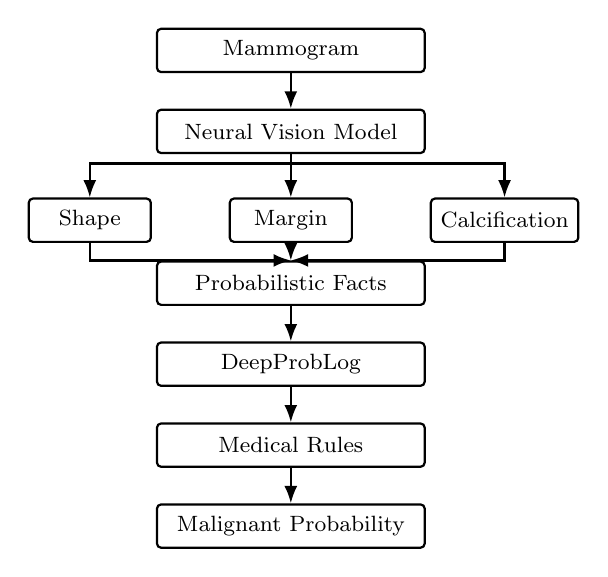
\begin{tikzpicture}[
  font=\footnotesize,
  node distance=0.45cm and 0.28cm,
  box/.style={
    draw,
    rounded corners=1.5pt,
    align=center,
    inner sep=3.5pt,
    minimum height=0.55cm,
    thick
  },
  concept/.style={
    box,
    minimum width=1.55cm
  },
  main/.style={
    box,
    minimum width=3.4cm
  },
  arr/.style={
    -{Latex[length=2.2mm]},
    thick
  }
]
  \node[main] (mammo) {Mammogram};
  \node[main, below=of mammo] (nn) {Neural Vision Model};
  \node[concept, below left=0.55cm and 0.05cm of nn] (shape) {Shape};
  \node[concept, below=0.55cm of nn] (margin) {Margin};
  \node[concept, below right=0.55cm and 0.05cm of nn] (calc) {Calcification};
  \node[main, below=1.35cm of nn] (facts) {Probabilistic Facts};
  \node[main, below=of facts] (dpl) {DeepProbLog};
  \node[main, below=of dpl] (rules) {Medical Rules};
  \node[main, below=of rules] (out) {Malignant Probability};

  \draw[arr] (mammo) -- (nn);
  \draw[arr] (nn.south) -- ++(0,-0.12) -| (shape.north);
  \draw[arr] (nn.south) -- (margin.north);
  \draw[arr] (nn.south) -- ++(0,-0.12) -| (calc.north);
  \draw[arr] (shape.south) |- (facts.north);
  \draw[arr] (margin.south) -- (facts.north);
  \draw[arr] (calc.south) |- (facts.north);
  \draw[arr] (facts) -- (dpl);
  \draw[arr] (dpl) -- (rules);
  \draw[arr] (rules) -- (out);
\end{tikzpicture}
\caption{Overview of the proposed neuro-symbolic breast cancer diagnosis framework. A neural vision model extracts concept-level evidence (e.g., shape, margin, and calcification), which is represented as probabilistic facts and reasoned over by DeepProbLog with medical rules to produce a malignant probability.}
\label{fig:architecture}
\end{figure}

\subsection{Neural Visual Concept Extraction}
\label{sec:concepts}

The neural model transforms raw image information into clinically meaningful visual concepts, each with an associated probability. Conceptually,
\begin{center}
\small
Image $\rightarrow$ CNN / Vision Model $\rightarrow$ $\{\mathrm{mass},\;\mathrm{margin},\;\mathrm{shape},\;\mathrm{calcification},\;\ldots\}$.
\end{center}
This differs from a direct mapping $\mathrm{Image}\rightarrow\mathrm{Malignant}$. The working concept inventory is lesion kind (mass vs.\ calcification), mass shape, mass margin, and calcification type. Other BI-RADS-aligned descriptors may be added where annotations permit~\cite{acr2013birads,lee2017cbis}. The study distinguishes among: (i)~concepts directly annotated in the dataset; (ii)~concepts derivable from metadata; and (iii)~concepts requiring additional annotation or modeling assumptions.

The diagnostic target is binary malignancy. In CBIS-DDSM the original pathology field typically has three values: malignant, benign, and benign-without-callback (benign with no additional follow-up indicated). Any label other than malignant is mapped to the negative class. This merges the two non-malignant categories and is a simplifying assumption, not a claim that those categories are clinically identical.
% TODO: Finalize concept inventory after dataset selection and annotation audit.
% TODO: Do not assume BUSI provides BI-RADS descriptor labels unless verified.
% TODO: For CBIS-DDSM, verify which BI-RADS descriptors are usable for supervision.

\subsection{Probabilistic Logic Representation}
\label{sec:problog}

Because concept extraction is imperfect, the symbolic component should reason over uncertain evidence rather than treating neural predictions as absolute truths. Neural outputs can be represented as probabilistic facts or neural predicates parameterized by the vision model~\cite{deraedt2007problog,manhaeve2018deepproblog}. DeepProbLog supplies probabilities from neural networks, applies logical rules relating concepts to diagnostic hypotheses, and computes the success probability of a diagnostic query. The motivation is joint handling of perception, uncertainty, probabilistic reasoning, and symbolic knowledge---not replacing ordinary conditionals with equivalent Prolog.

\subsection{Medical Knowledge and Rule Representation}
\label{sec:knowledge}

The symbolic knowledge base will be constructed from verified domain knowledge and, where applicable, BI-RADS terminology and assessment criteria~\cite{acr2013birads}. Exact rules will be defined only after verifying the relevant clinical documentation. This paper does not invent diagnostic rules or present unverified heuristics as official BI-RADS guidelines.
% TODO [REQUIRES CLINICAL VERIFICATION]: Define the symbolic rule set from primary BI-RADS documentation and/or clinician-validated knowledge.
% TODO: Decide whether the target is binary malignancy, BI-RADS assessment categories, or an intermediate risk formulation.

The symbolic layer is intended to provide explicit structure, traceable decision paths, and separation between learned perception and declarative knowledge. Whether this improves diagnostic performance remains an experimental question.

\subsection{Neuro-Symbolic Inference}
\label{sec:inference}

The neural model learns concept predictors from images; the symbolic model encodes domain knowledge; and DeepProbLog combines probabilistic neural outputs with logical reasoning~\cite{manhaeve2021neural}. Depending on the formulation, gradients may propagate through probabilistic reasoning to optimize the neural component. This possibility will be investigated, but is not assumed to be automatically beneficial. The goal is neural learning combined with symbolic knowledge and probabilistic reasoning, not deterministic Prolog alone. Reasoning traces may support interpretability, but do not by themselves guarantee clinically adequate explanations.

\section{Experimental Setup}
\label{sec:experiments}

Unless marked otherwise, the choices below are provisional.

\subsection{Dataset}
\label{sec:dataset}

Two public datasets are currently considered:
\begin{itemize}
\item \textbf{BUSI:} Breast ultrasound images labeled as normal, benign, or malignant, with mask annotations~\cite{aldhabyani2020busi}.
\item \textbf{CBIS-DDSM:} Curated mammography cases with pathology information and, for many abnormalities, BI-RADS-related descriptors such as mass shape/margin and calcification type/distribution~\cite{lee2017cbis}. The current implementation uses CBIS-DDSM.
\end{itemize}
Mass and calcification tables are merged. After that merge, some patients appear in both official train and test splits; those patients are assigned entirely to train so that evaluation remains patient-disjoint. As stated in Section~\ref{sec:concepts}, pathology is reduced to a binary label by treating benign and benign-without-callback as a single negative class. This is a simplifying assumption. Selection of any additional dataset will depend on label availability, image quality, class distribution, concept-relevant annotations, and compatibility with the proposed representation.
% TODO: Select the primary dataset; report splits, class counts, preprocessing, and exclusion criteria.

\begin{table}[!t]
\caption{Dataset characteristics (to be completed after final selection).}
\label{tab:dataset}
\centering
\small
\begin{tabular}{@{}lccc@{}}
\toprule
Dataset & Modality & Samples & Concept labels \\
\midrule
BUSI~\cite{aldhabyani2020busi} & Ultrasound & \todo{N} & \todo{verify} \\
CBIS-DDSM~\cite{lee2017cbis} & Mammography & \todo{N} & \todo{verify} \\
\bottomrule
\end{tabular}
\end{table}

\subsection{Neural Model}
\label{sec:neural}

Candidate backbones include a standard CNN baseline and residual networks such as ResNet~\cite{he2016resnet}; alternatives may be considered. Geometric augmentation (horizontal flip, small rotation, and mild affine perturbation) is applied to training images only; validation and test images are left unchanged. Learning rate and batch size are selected by a small grid search on validation macro F1, after which the selected pair is used for the full training run.
Two neural roles are planned: an end-to-end diagnostic classifier (baseline) and a concept extractor for the neuro-symbolic pipeline.

\subsection{DeepProbLog Configuration}
\label{sec:dplconfig}

The planned configuration includes neural predicates for lesion kind, shape, margin, and calcification type; probabilistic facts from those network outputs; symbolic rules that gate mass evidence and calcification evidence by lesion kind; and a diagnostic query for malignancy probability. These rules are a computational working program and are not presented as official BI-RADS criteria.
% TODO: Specify the final program, predicate signatures, query, learning schedule, and inference settings.

\subsection{Baselines}
\label{sec:baselines}

\begin{itemize}
\item \textbf{Baseline 1:} Pure neural image classifier.
\item \textbf{Baseline 2:} Neural concept-level model without DeepProbLog, if annotations permit (e.g., concept-bottleneck style)~\cite{koh2020concept}.
\item \textbf{Proposed:} Neural concepts + DeepProbLog + symbolic medical knowledge.
\end{itemize}

\subsection{Evaluation Metrics}
\label{sec:metrics}

The evaluation will report accuracy, precision, recall/sensitivity, specificity, F1-score for both classes (and their macro average), and ROC-AUC where applicable, with emphasis on sensitivity and specificity. Reporting only malignant F1 would hide a model that predicts a single class. Interpretability will be assessed qualitatively via reasoning traces on selected true/false positive and negative cases; expert review may be added if resources permit.
% TODO: Define the interpretability annotation protocol.

\section{Results and Discussion}
\label{sec:results}

Experimental results are not yet available. No performance numbers are reported here. The following subsections will be completed after the planned experiments.

\subsection{Quantitative Results}
[TO BE COMPLETED AFTER EXPERIMENTS]

Table~\ref{tab:comparison} will summarize baseline and proposed-model performance, emphasizing sensitivity and specificity in addition to accuracy, F1-score, and ROC-AUC.

\begin{table}[!t]
\caption{Comparison of baseline and neuro-symbolic models (placeholder).}
\label{tab:comparison}
\centering
\small
\begin{tabular}{@{}lcccc@{}}
\toprule
Model & Acc. & Sens. & Spec. & F1 \\
\midrule
Neural baseline & --- & --- & --- & --- \\
Concept neural baseline & --- & --- & --- & --- \\
Proposed (DeepProbLog) & --- & --- & --- & --- \\
\bottomrule
\end{tabular}
\end{table}

\subsection{Comparison with Neural Baselines}
[TO BE COMPLETED AFTER EXPERIMENTS]

This subsection will discuss whether the neuro-symbolic model improves, matches, or underperforms the neural baselines. Accuracy improvement remains a research hypothesis.

\subsection{Interpretability and Error Analysis}
[TO BE COMPLETED AFTER EXPERIMENTS]

Planned analyses include inspection of reasoning traces for selected cases, assessment of concept-prediction failures that propagate into symbolic inference, and identification of settings where medical knowledge constraints help or hurt the final decision. Availability of an explicit trace will be distinguished from clinical adequacy of that trace.

\section{Conclusion}
\label{sec:conclusion}

This paper presented a research framework for neuro-symbolic breast cancer diagnosis that combines neural visual concept extraction with DeepProbLog-based probabilistic logical reasoning and medical knowledge inspired by BI-RADS. The motivation is that purely end-to-end neural classifiers, while often effective, may not expose an explicit intermediate reasoning process suitable for clinical scrutiny. By estimating clinically meaningful visual concepts and reasoning over their uncertainty within a probabilistic logic program, the proposed approach aims to support more interpretable diagnostic decision structures and a clearer separation between learned perception and explicit domain knowledge.

The neural component is responsible for perception; DeepProbLog provides the mechanism for uncertain symbolic inference; and the knowledge base is intended to encode verified medical criteria rather than ad hoc rules. The planned evaluation will compare the proposed pipeline against conventional neural baselines using standard diagnostic metrics and qualitative analysis of reasoning traces. Because experiments have not yet been completed, this work does not claim improved accuracy, clinical readiness, or guaranteed explainability.

Future work includes validation on additional datasets, refinement of the concept inventory, enrichment of clinically verified knowledge, expert evaluation of reasoning traces, and robustness testing under distribution shift and incomplete concept supervision.


\bibliographystyle{IEEEtran}
\bibliography{references}

\end{document}
